%%%%%%%%%%%%%%%%%%%%%%%%%%%%%%%%%%%%%%%%%%%%%%
%                insertmeeting
% 1) Title (something creative & funny?)
% 2) Date (MM/DD/YYYY)
% 3) Location (ex. Hagerty High School)
% 4) People/Committees Present 
% 5) Picture 
% 6) Start Time & Stop Time (ex. 12:30AM to 4:30PM)
%%%%%%%%%%%%%%%%%%%%%%%%%%%%%%%%%%%%%%%%%%%%%%
\insertmeeting 
	{Busy Days} 
	{10/29/21}
	{Hagerty High School}
	{Annika, Anouska, Jensen, Nathan, Ritam, Samantha}
	{Images/RobotPics/robot.jpg}
	{2:30 - 4:30}
	
\hhscommittee{General}
\noindent\hfil\rule{\textwidth}{.4pt}\hfil
\subsubsection*{Goals}
\begin{itemize}
    \item Driver Practice
    \item Creating a forcefield for the arm
    \item Figuring out the mathematical model for the differential 

\end{itemize} 

\noindent\hfil\rule{\textwidth}{.4pt}\hfil

\subsubsection*{Accomplishments}
After the hardware committee finished testing and fixing the drivetrain, we initiated some driver practice so that the people who were wanting to drive could have practice for the meet coming up on November 13th. Turns out, we weren’t that great at driving, however the old saying “practice makes perfect” applies here, and with more practice we are sure to get better. Afterwards, we started working on a little bit of software to help aid the driver. We had recently added a PID control algorithm to our arm mechanism to go perpendicular to the ground for the following 2 reasons: the arm reaching outside the playing area, and stopping the arm before it rams into the plate that stops the arm itself. The arm reaching outside the playing area was an issue at first because when we turned towards the warehouse, the arm would constantly be across the field barrier which would result in a penalty. The other issue about the arm ramming into the plate was important because at times the yellow cube would fall out of our intake grabbing mechanism when it hit the plate so hard. The PID algorithm would aid in stopping the arm a bit before it hit the plate and then letting gravity let it fall from there. By just allowing gravity to let it fall, it would reduce the impact it had on the plate, thus the block not falling out of our intake mechanism. We tested this idea and found that it worked really well, however our P value in the PID controller was too low for the arm to be able to get it back to a perpendicular position which caused an issue in that it would sometimes be towards the side where we intake and fall back down when we drove forward. As a solution, we decided to create a forcefield where every time it got past its perpendicular position, the PID would activate, not allowing the arm to fall all the way down as there would be power every single time it did. This ended up working well, however we think it will be better if we create 2 buttons for it to be perpendicular to the ground and another for going super close to the plate that’s supposed to stop it so that it would just barely have any force. This will allow the block to not fall out even if it's barely clutched in with the grabber. After working on all the PID controls with the arm, we started working on the mathematical model of the differential equation we found yesterday. We created a method in HhsTricycleDriveBase called getDifferentialRatio. This will give us the ratio between the path created by the middle of the robot when it goes at a certain angle + the distance between the wheels and the center of the robot and the path created by the middle of the robot - the distance between the wheels. We would then take that ratio and use that same ratio for the motor powers so that the robot won’t skid. However, this caused another issue. We wanted the middle of the robot to be going at the same speed (as it will then go off the original middle circle), which means the velocity of the outer circle and inner circle needed to have the ratio coefficient we found earlier but also have the same ratios from the middle circle. We were unable to figure this part out, however we created some of our own formulas to help figure out the motor powers so that the middle circle would stay the same.

\begin{figure}[htp]
\centering
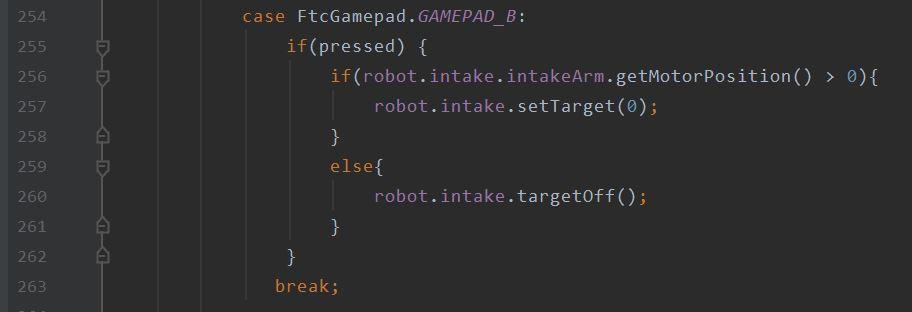
\includegraphics[width=0.95\textwidth, angle=0]{Meetings/October/10-29-21/armForcefield - Ritam R.JPG}
\caption{Code to control the arm.}
\label{fig:102921_1}
\end{figure}

\begin{figure}[htp]
\centering
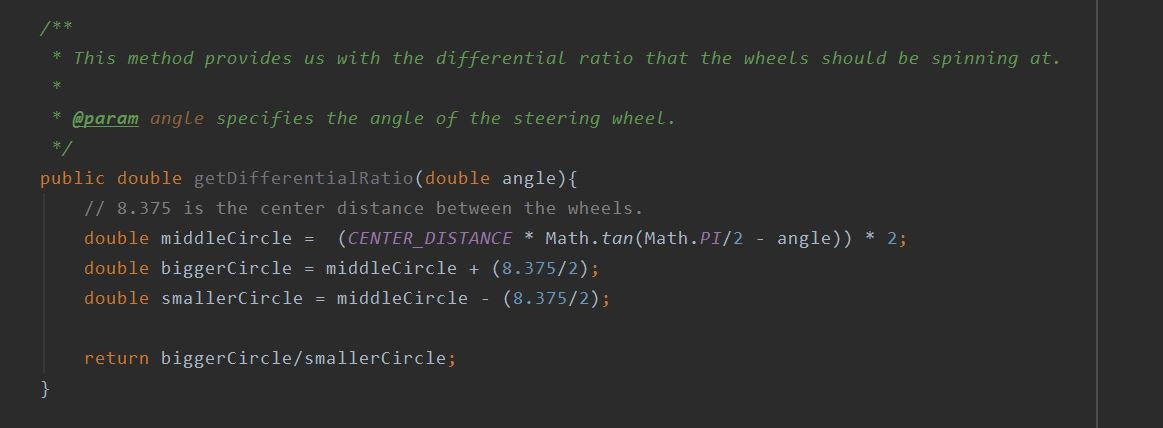
\includegraphics[width=0.95\textwidth, angle=0]{Meetings/October/10-29-21/getDifferentialRatio - Ritam R.JPG}
\caption{Our method to calculate a differential ratio for the wheels.}
\label{fig:102921_2}
\end{figure}


\hhscommittee{CAD}
\noindent\hfil\rule{\textwidth}{.4pt}\hfil
\subsubsection*{Goals}
\begin{itemize}
    \item Design arm plan from yesterday’s meeting

\end{itemize} 

\noindent\hfil\rule{\textwidth}{.4pt}\hfil

\subsubsection*{Accomplishments}
Following the meeting yesterday, us CAD committee members have been thinking about this new arm design. Today, we jumped into cad, eager to start designing. We started off by designing the 3d printed slider joints, as they would determine how the rest of the arm would go together. Looking at the old design, we noticed that there were 2 different types of holes on the 3D printed parts, one type that firmly held the carbon fiber rods for structure and another type that allowed the carbon fiber rods to smoothly slide through. For our design, we decided to use 2 a similar strategy, but we wanted to use different diameter rods for increased support running the length of the arm, in the direction where the arm will be the longest and skinniest. We decided on rod diameters of .25 inches for the horizontal and .30 inches for the vertical. With these sizes decided, we created the main slide joints (Figure \ref{fig:102921_3}). Each of these joints has 3 holes, one for the horizontal rods and 2 for the vertical rods. The holes for the vertical rods, like we observed on the old design, are 2 different sizes, one that will hold the rods firmly, and one that has a slight offset from the .3 inch rod diameter that will allow the carbon fiber to slide through it. 
Although our design has many of the same basic ideas as the ould lift from a previous season, we improved upon it using our more advanced design skills that allowed us to create stronger yet lighter joints. As we have learned this year, creating a smaller, shell like design then adding ribs for support can create a much more efficient and well rounded part. Although these parts are small and may seem insignificant, ensuring that we make every part of our robot as well as we can is very important to all of our members-- and these joints are no exception. An approximation of the old design compared to our new one is shown in Figure \ref{fig:102921_4}.
To make sure that everything in our design is solid, we recreated the carbon fiber rods and combined them with the joints in an assembly. Using slider mates and adding limits, we were able to realistically simulate how the arm would slide (Figures \ref{fig:102921_5} and \ref{fig:102921_6}). With everything in the assembly, we could verify that all of the parts worked together as expected!


\begin{figure}[ht]
\centering
\begin{minipage}[b]{.48\textwidth}
  \centering
  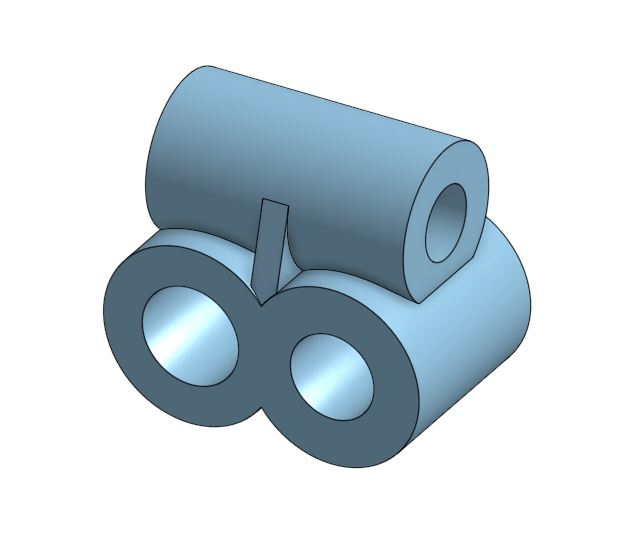
\includegraphics[width=0.95\textwidth]{Meetings/October/10-29-21/10-29-21_CAD_Figure1 - Nathan Forrer.JPG}
  \caption{The main slide joints.}
  \label{fig:102921_3}
\end{minipage}%
\hfill%
\begin{minipage}[b]{.48\textwidth}
  \centering
  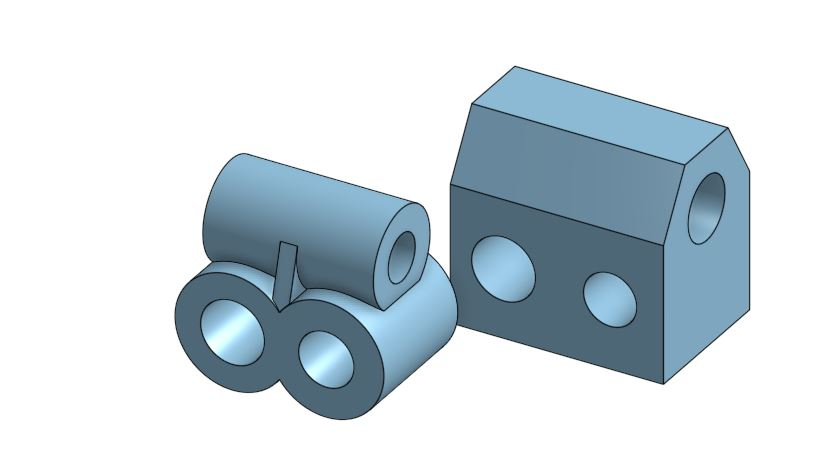
\includegraphics[width=0.95\textwidth]{Meetings/October/10-29-21/10-29-21_CAD_Figure2 - Nathan Forrer.JPG}
  \caption{Old design vs. new design.}
  \label{fig:102921_4}
\end{minipage}
\end{figure}

\begin{figure}[ht]
\centering
\begin{minipage}[b]{.48\textwidth}
  \centering
  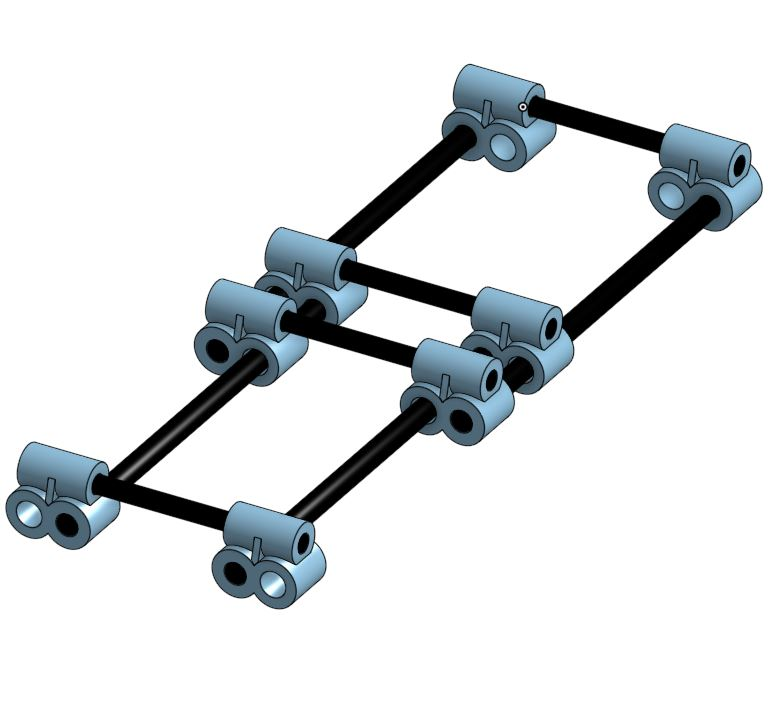
\includegraphics[width=0.95\textwidth]{Meetings/October/10-29-21/10-29-21_CAD_Figure3 - Nathan Forrer.JPG}
  \caption{CAD of compressed arm.}
  \label{fig:102921_5}
\end{minipage}%
\hfill%
\begin{minipage}[b]{.48\textwidth}
  \centering
  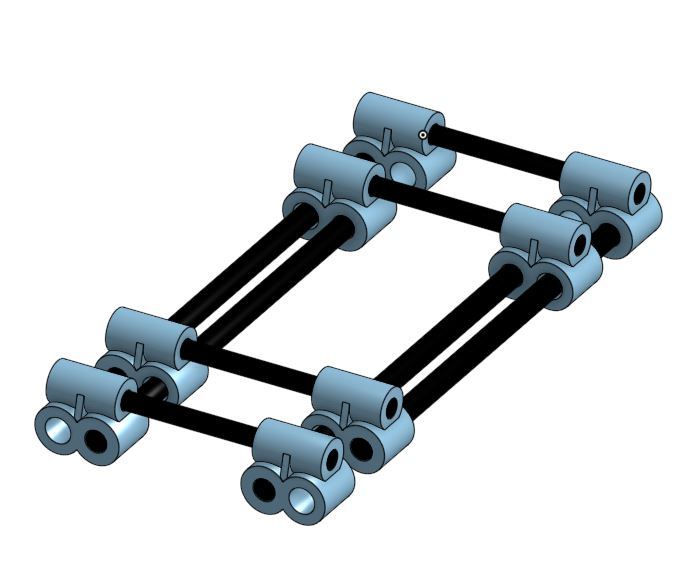
\includegraphics[width=0.95\textwidth]{Meetings/October/10-29-21/10-29-21_CAD_Figure4 - Nathan Forrer.JPG}
  \caption{CAD of extended arm.}
  \label{fig:102921_6}
\end{minipage}
\end{figure}

\hhscommittee{Hardware}
\noindent\hfil\rule{\textwidth}{.4pt}\hfil
\subsubsection*{Goals}
\begin{itemize}
    \item Attach belts to drivetrain
	\item Test drivetrain


\end{itemize} 

\noindent\hfil\rule{\textwidth}{.4pt}\hfil

\subsubsection*{Accomplishments}
Now that our new belt has arrived for the drivetrain, we were able to finish building and were ready to test how this new drivetrain maneuvers. We started by attaching the belts to the pulleys on the drivetrain (Figure \ref{fig:102921_7}). With most of the hardware put together for the drivetrain, we started attaching the electronics like the rev hub and the battery. To save space, we placed the battery below the rev hub, where it will stay secured with some velcro straps. The rev hub is held onto the drivetrain with standoffs that are long enough to allow the battery to easily slide underneath it. Then, after adding the wire and doing basic wire management, we were ready to test the robot.
After we had driven around for a few minutes one thing was clear: this drivetrain didn’t handle well. To start with, whenever we would start moving forward, the robot would jerk violently, raising the front wheel off the floor for a second or two before touching back on the ground. Although this seems like a cool trick the robot is able to do, it really just inhibits our ability to control the robot's steering. Because we steer from the front wheel, whenever the front wheel is off the ground, the robot is essentially out of control, making small movements near impossible. We thought about our test car drive from a few weeks back and wondered why this problem wasn’t present. As it turned out, our problem was simply that the new drivetrain’s weight distribution was farther back than the test drivetrain. For that one, we had placed the battery, which is the heaviest single component of the robot, right at the front over the front wheel. This weighed the robot down significantly, preventing the wheelie issue we are facing now. We were able to solve this by putting the battery in front of the arm (Figure \ref{fig:102921_9}), where its weight is now much farther in front of the two back wheels. When we tested this solution, we found that the robot barely jumped up anymore, significantly improving the robot’s steering.
The other problem we observed was only when we were making very tight turns. As we steered the robot sharply to either, the back wheels would drag against the ground as if they didn’t want to turn with the rest of the robot. Once again, this was a problem we hadn’t seen with the test car drive, which we determined is due to the increased width of this drivetrain. Because the back wheels are farther apart than before, they must move sideways more around sharp turns. Because the back wheels aren't controlling turning like in a typical tank drive, they must drag to allow the robot to turn, and the added width of the wheels made the dragging much more noticeable. This is a much more difficult problem to solve than weight distribution and will most likely need a software fix. After discussing with software, we determined that the best solution would be to create a program that acts like a differential on a car by slowing down one of the wheels as the robot turns. This will allow the robot to turn smoother by emulating how a typical tank drive might turn, while preserving the robust steering technique employed by the front wheel.



\begin{figure}[ht]
\centering
\begin{minipage}[b]{.48\textwidth}
  \centering
  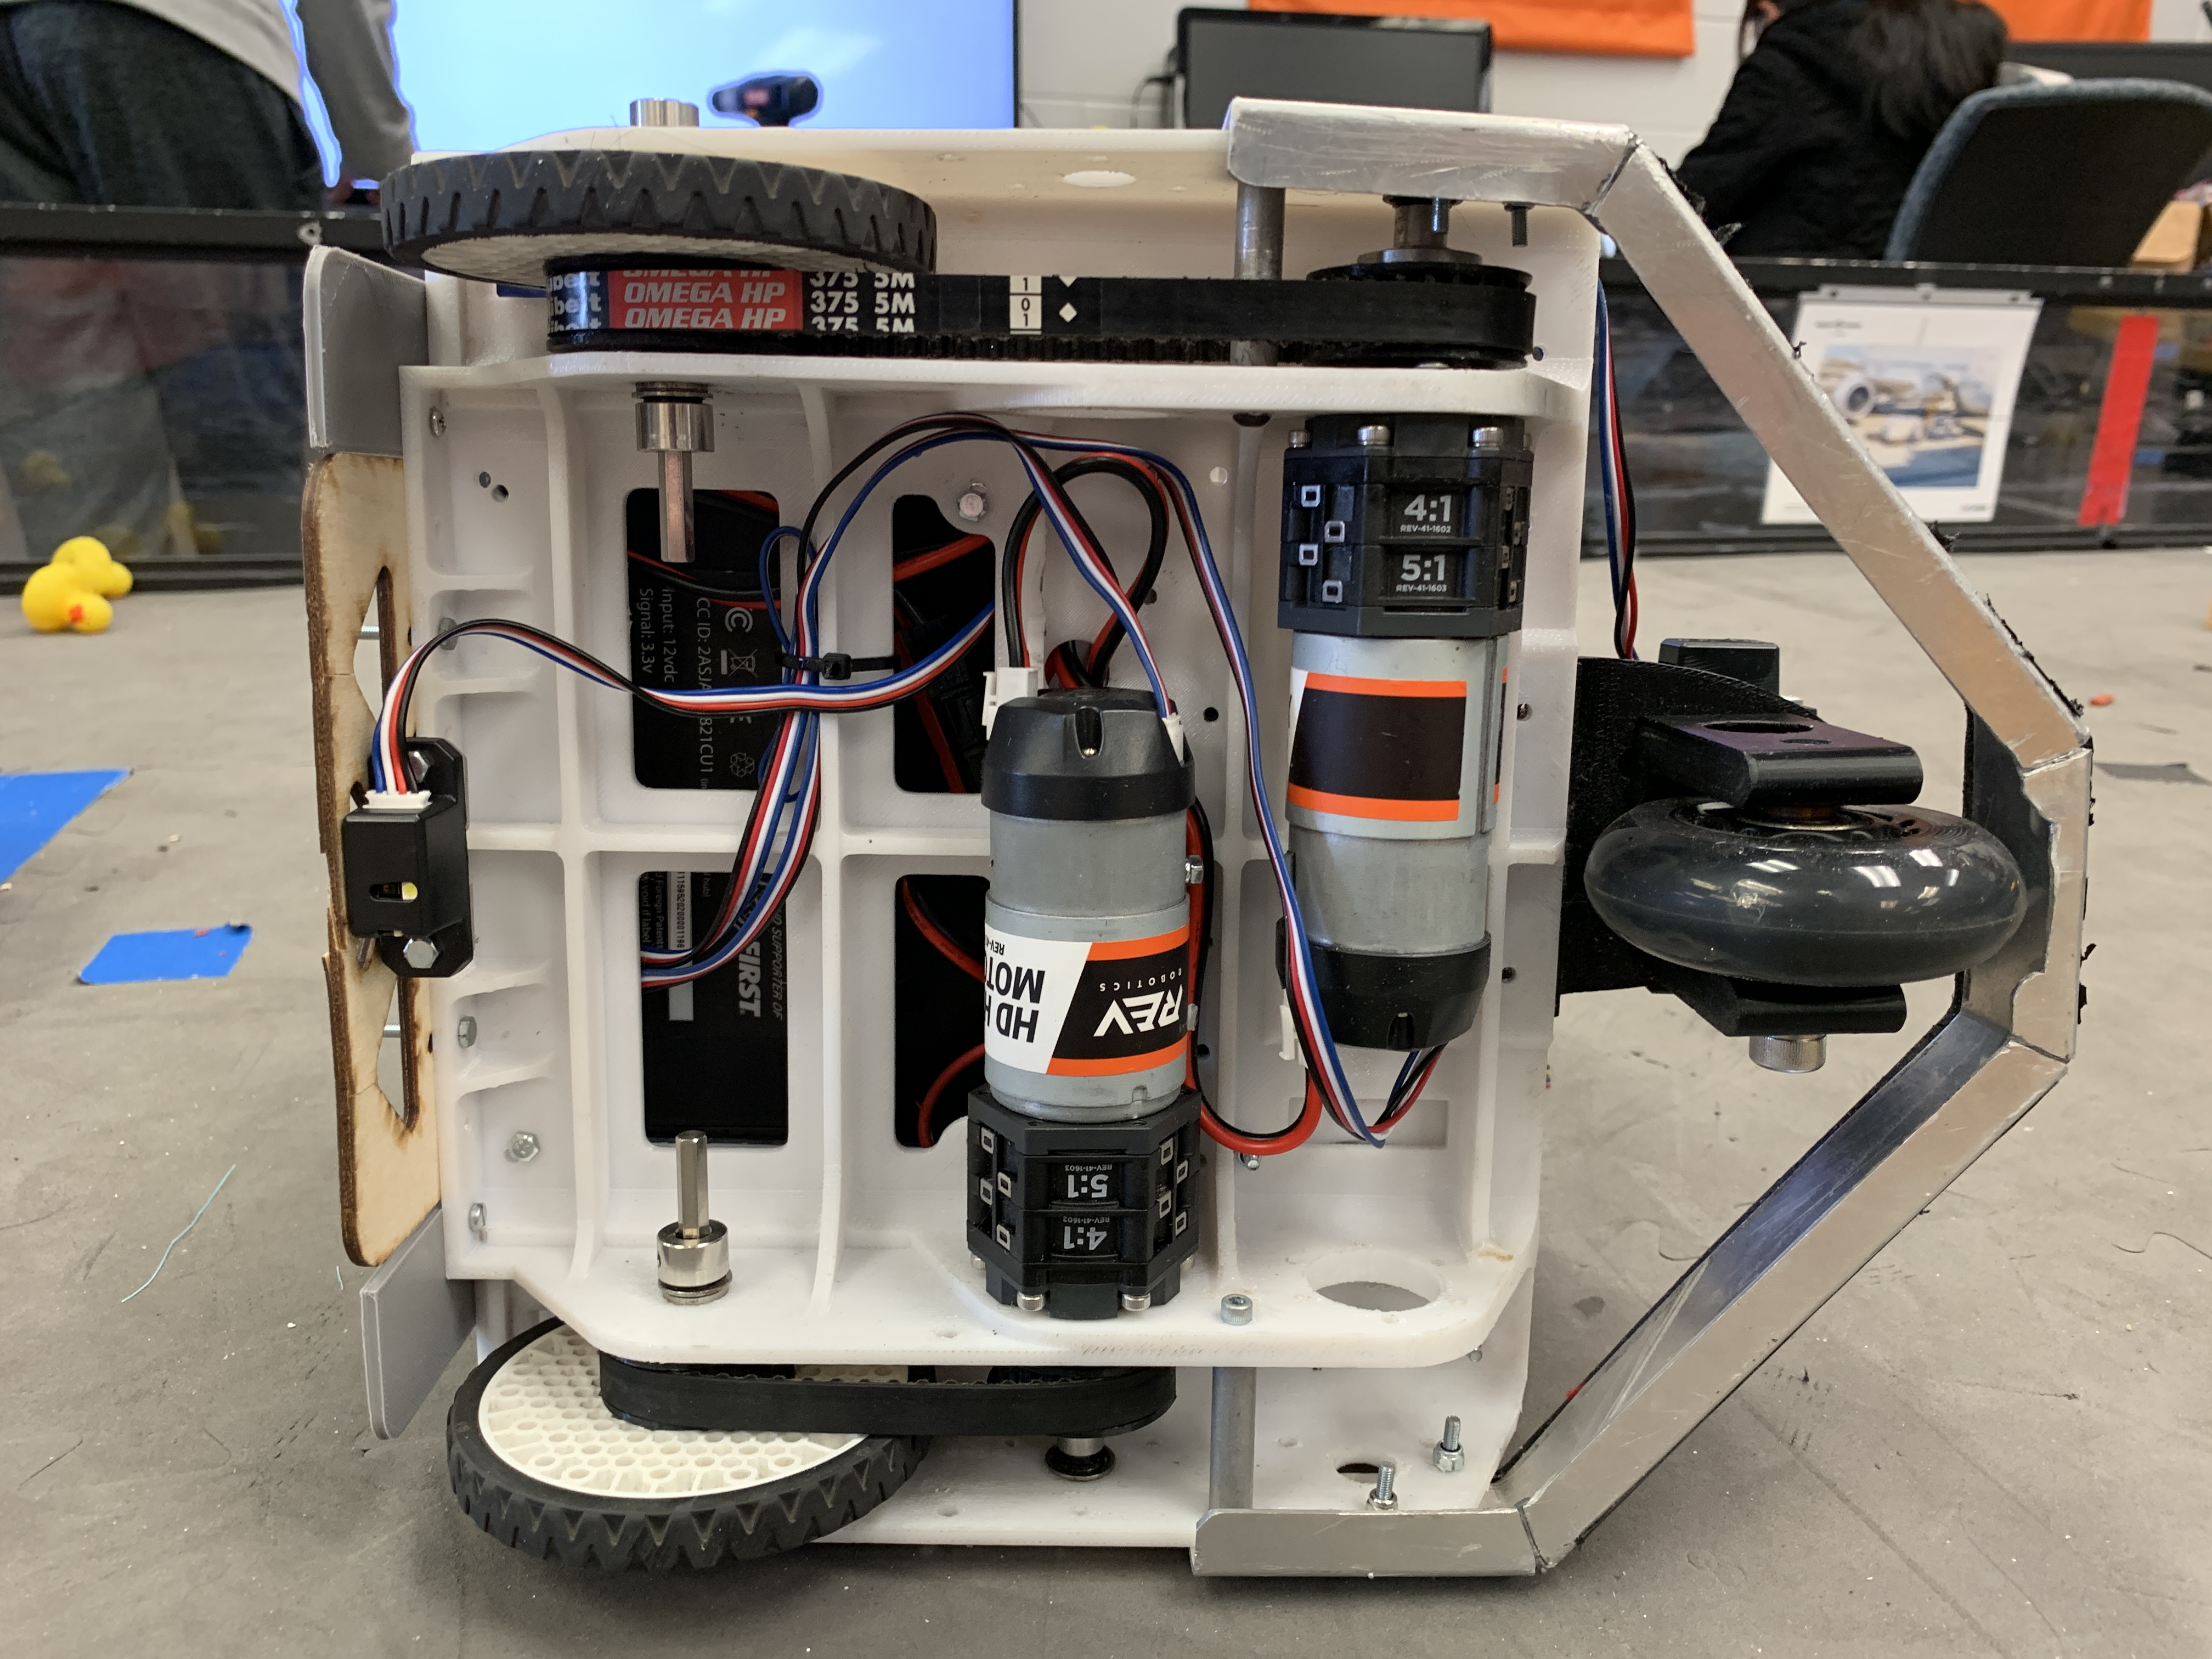
\includegraphics[width=0.95\textwidth]{Meetings/October/10-29-21/10-29-21_Hardware_Figure1 - Nathan Forrer.JPG}
  \caption{Attached belts.}
  \label{fig:102921_7}
\end{minipage}%
\hfill%
\begin{minipage}[b]{.48\textwidth}
  \centering
  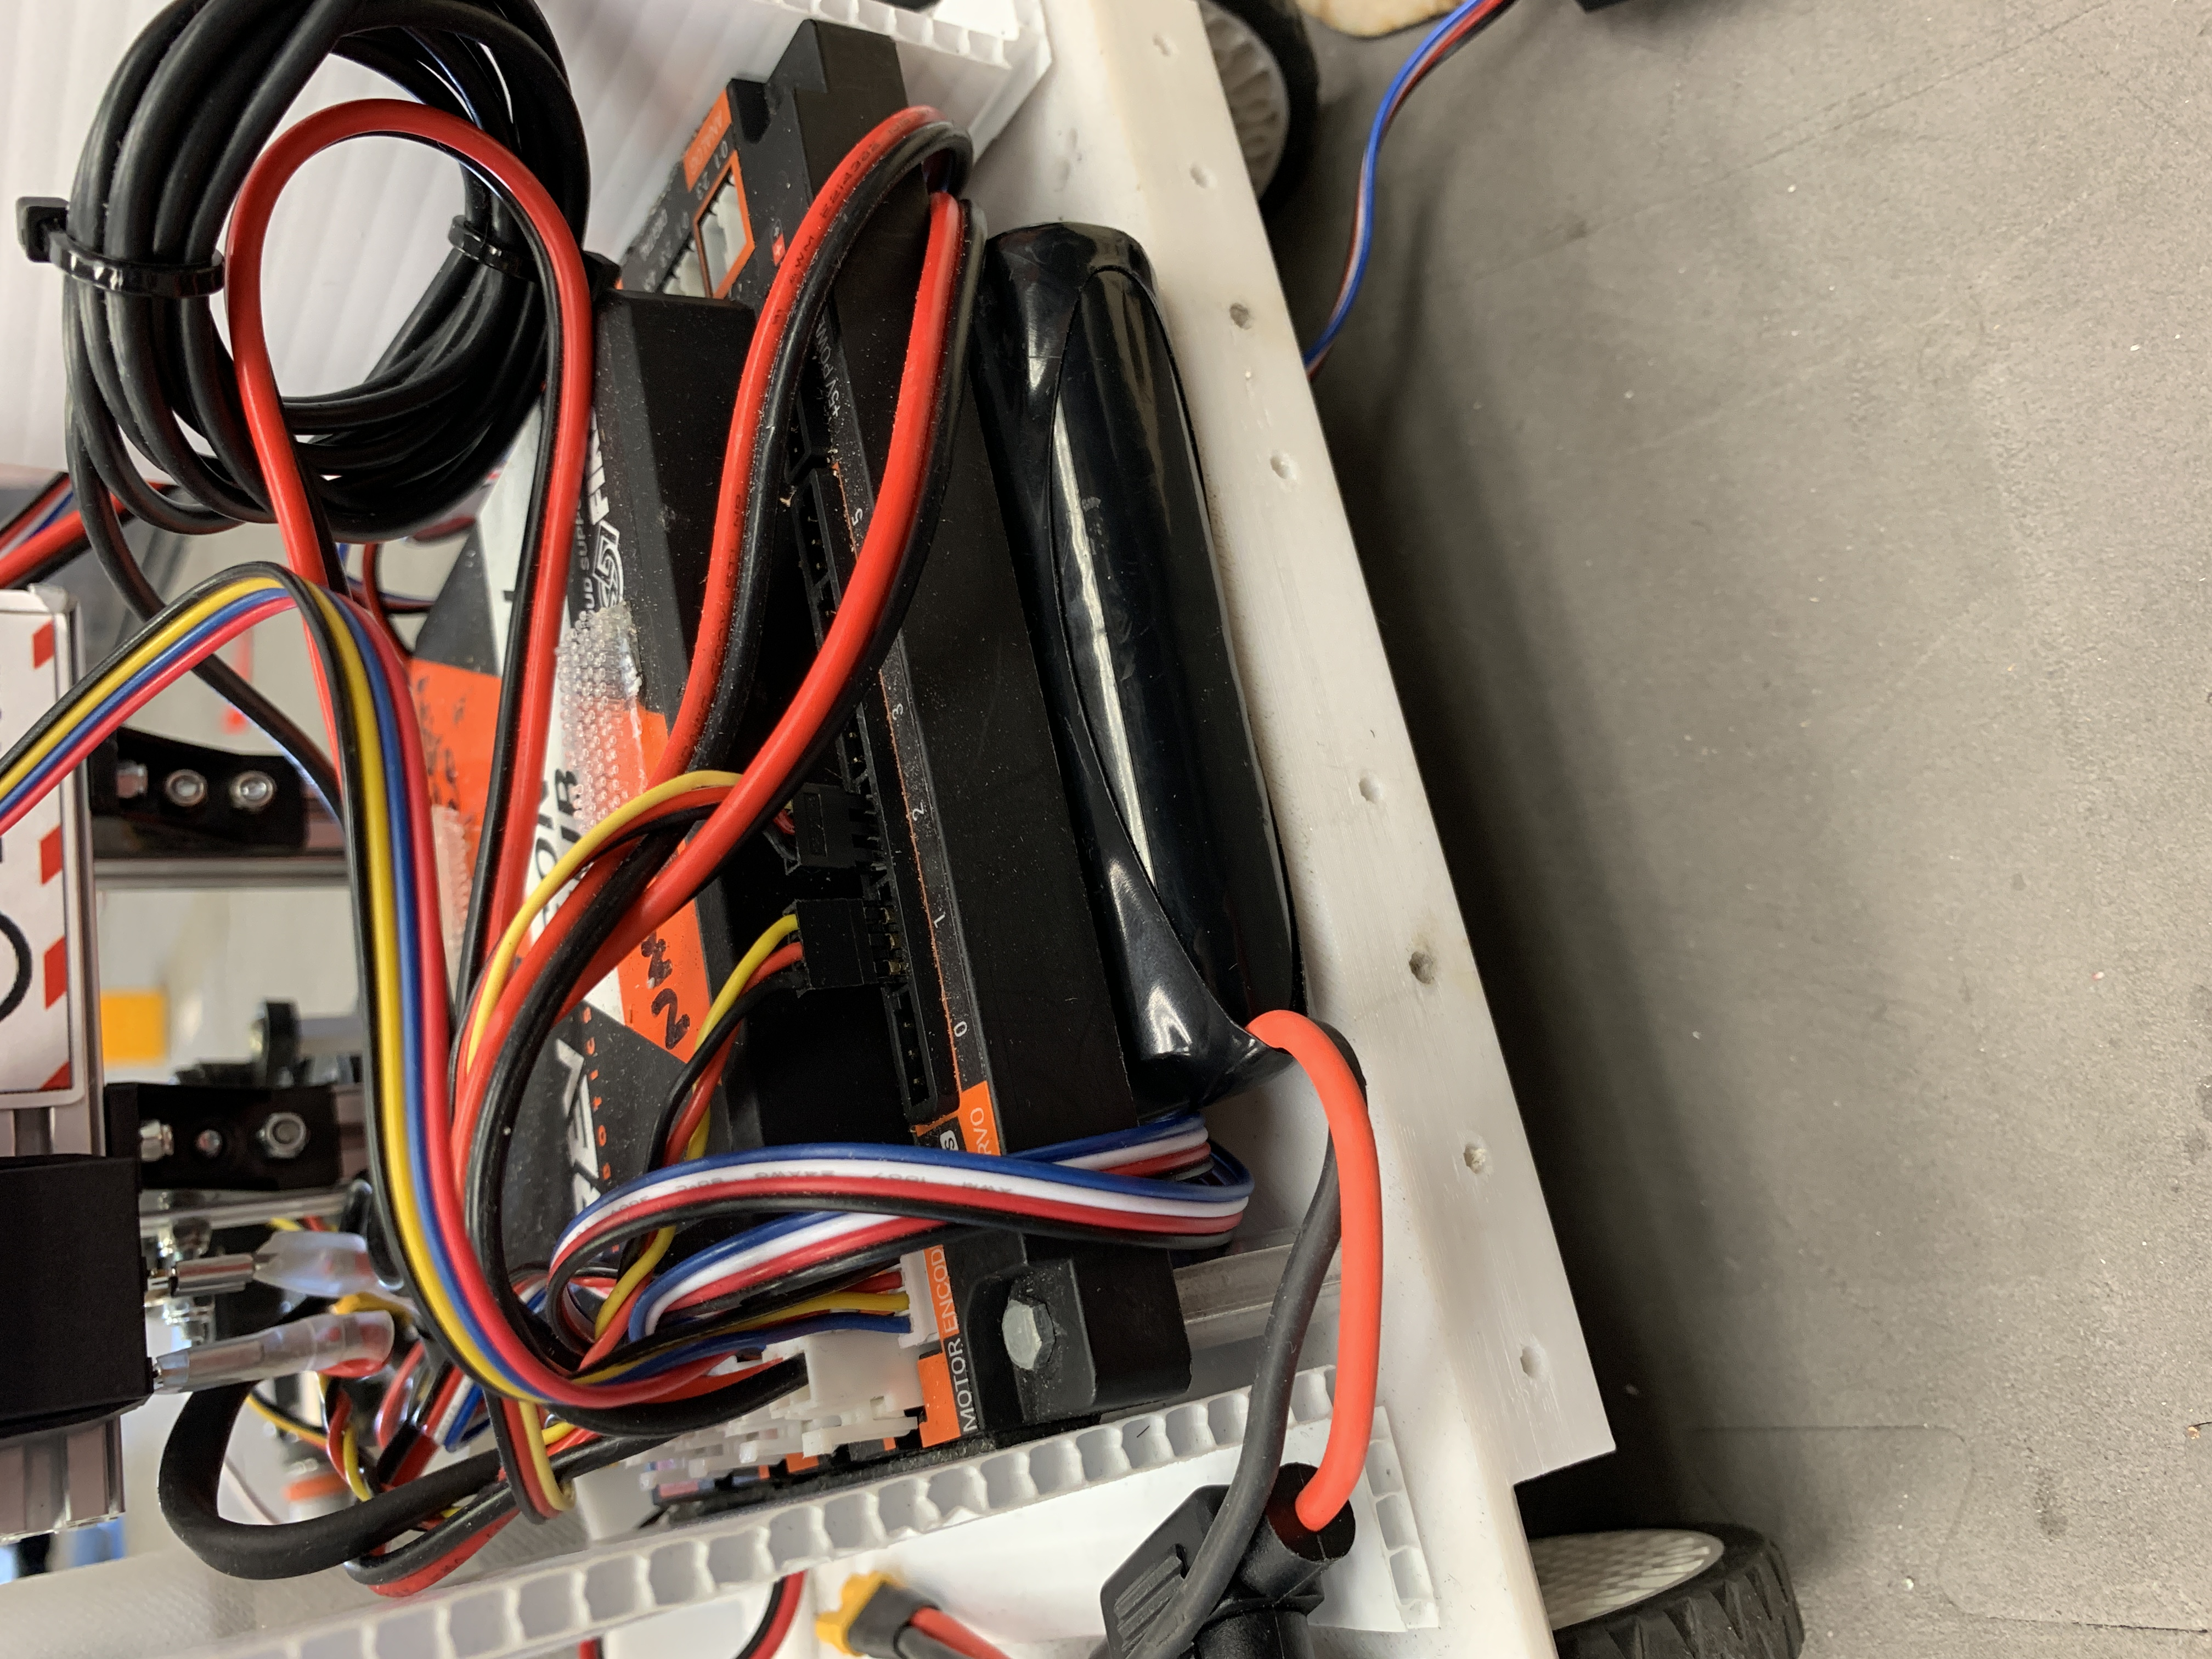
\includegraphics[width=0.95\textwidth]{Meetings/October/10-29-21/10-29-21_Hardware_Figure2 - Nathan Forrer.JPG}
  \caption{RevHub placement.}
  \label{fig:102921_4}
\end{minipage}
\end{figure}

\begin{figure}[htp]
\centering
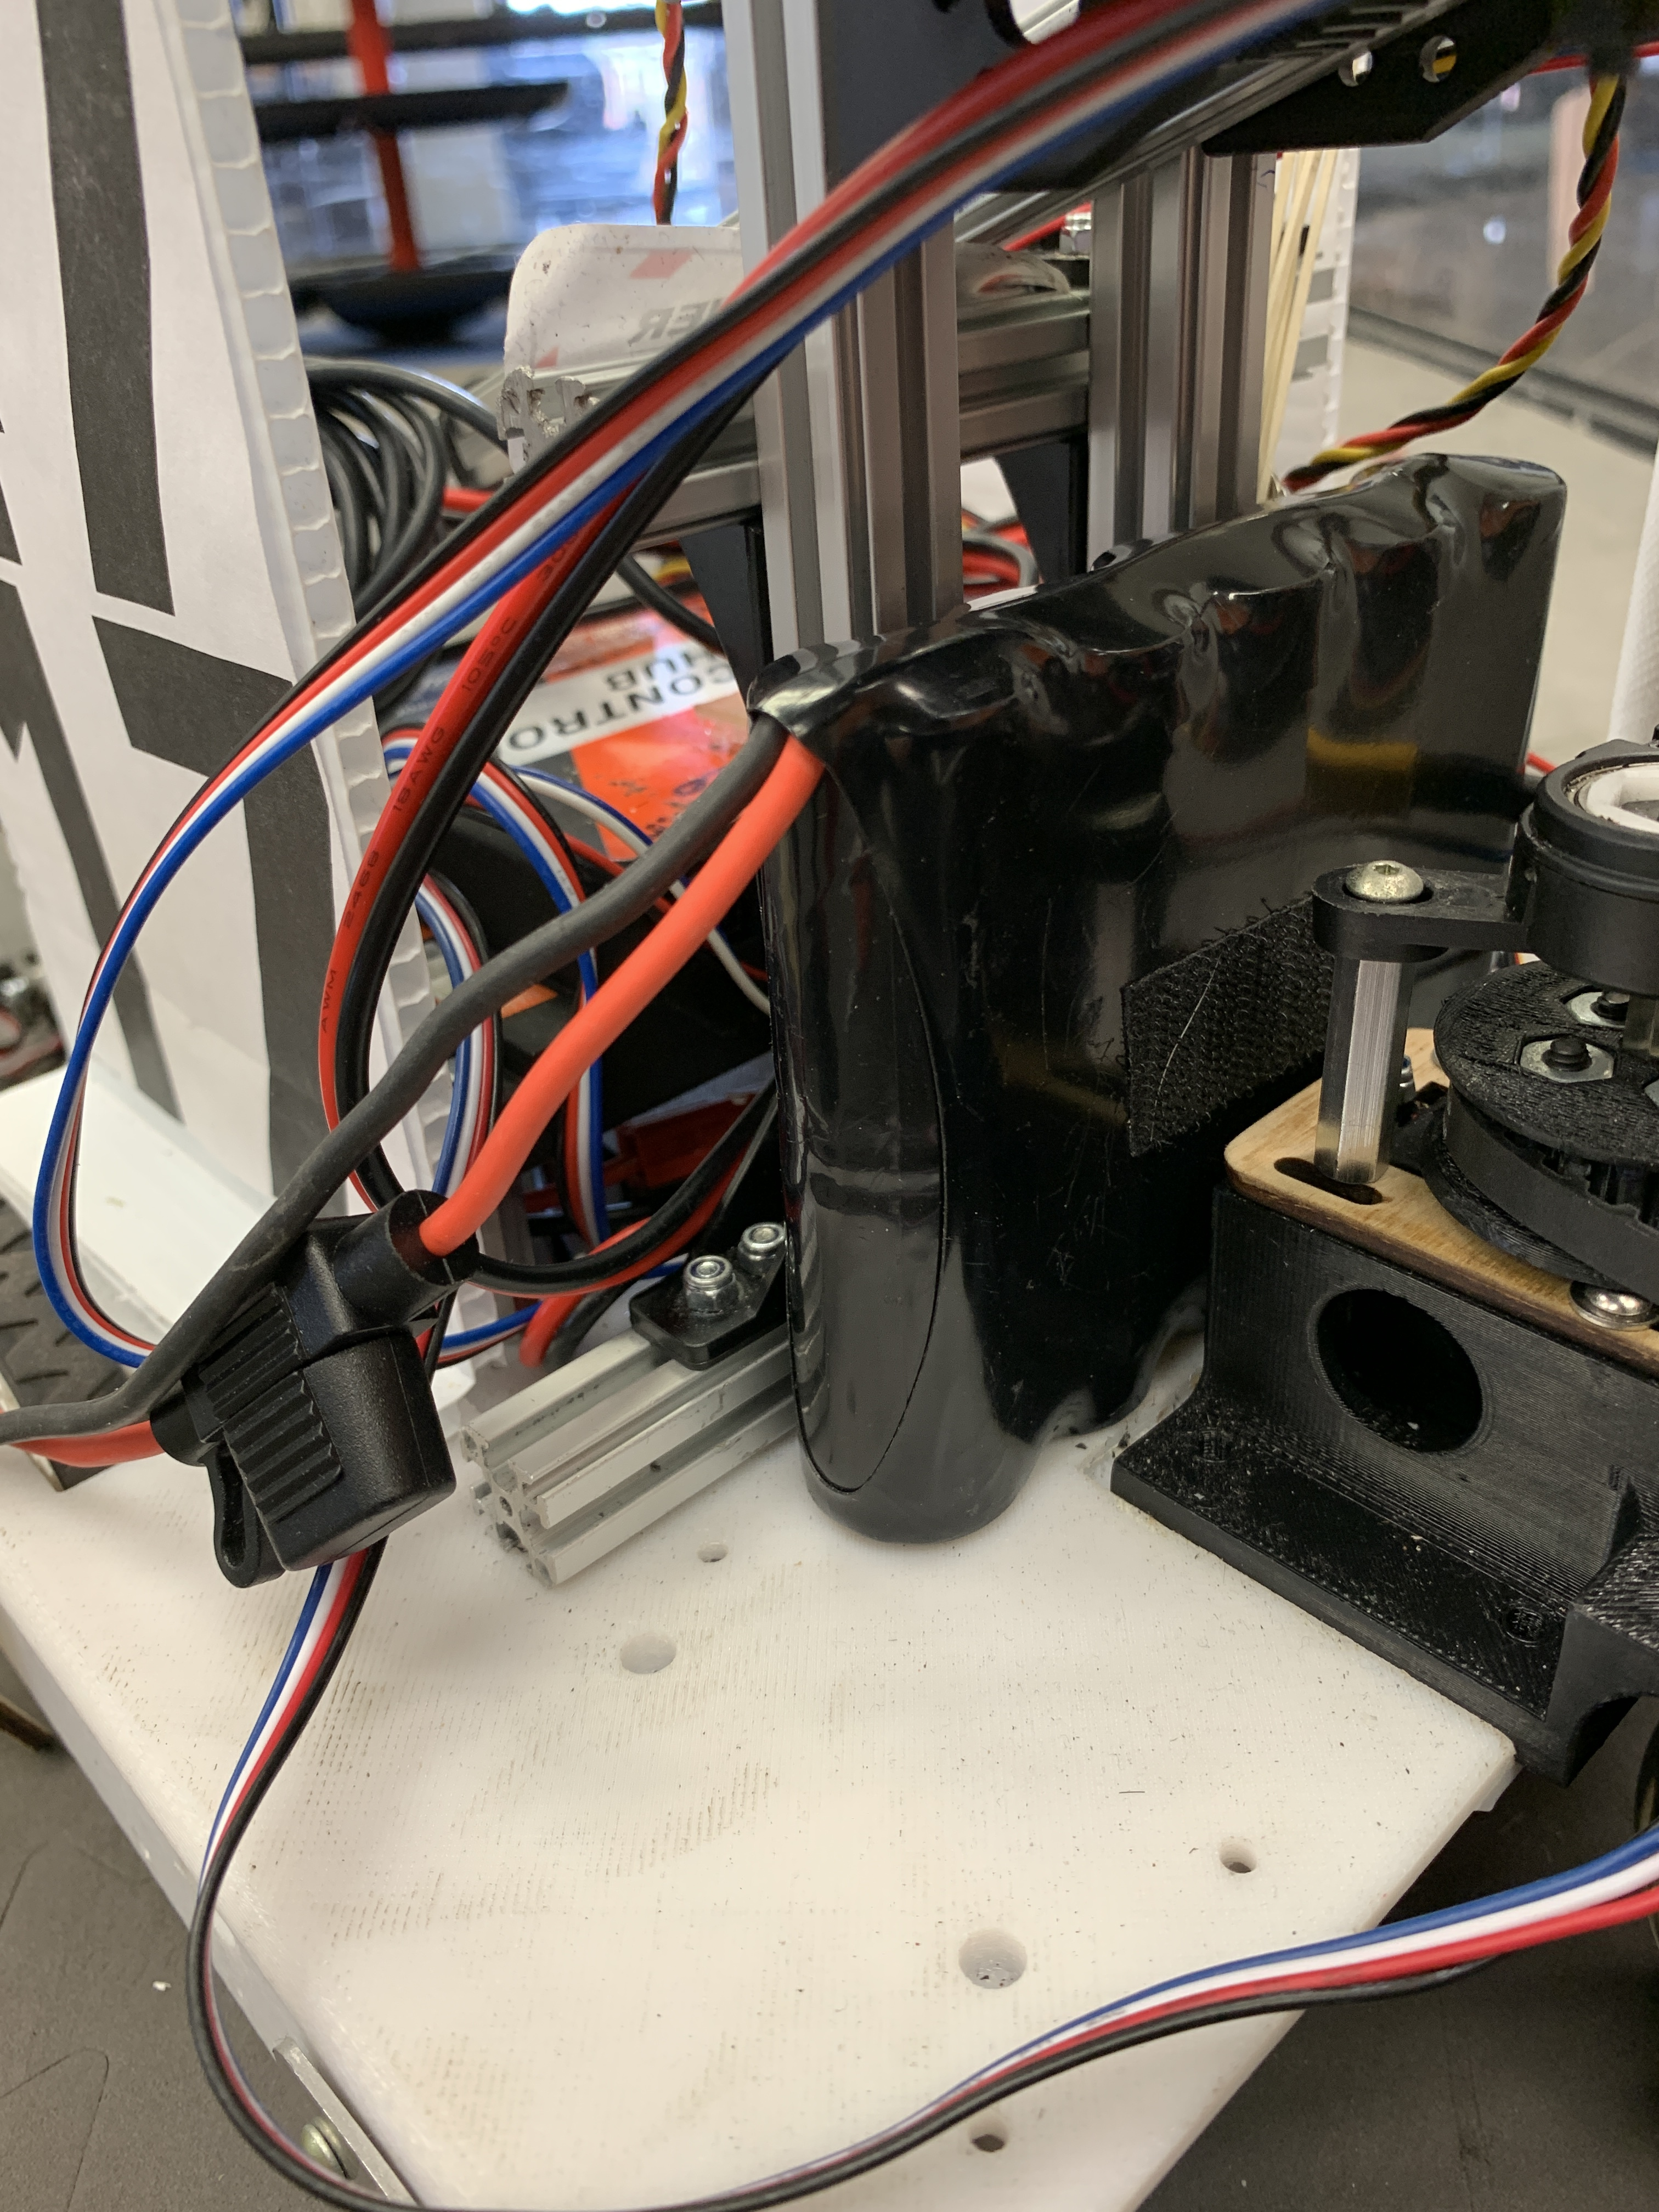
\includegraphics[width=0.95\textwidth, angle=0]{Meetings/October/10-29-21/10-29-21_Hardware_Figure3 - Nathan Forrer.JPG}
\caption{Moving the battery near the arm.}
\label{fig:102921_9}
\end{figure}


\whatsnext{
\begin{itemize}
    \item Finish up the differential method and test
    \item Set a PID on the angle of the wheel and the Y distance for autonomous
    \item Use Vuforia pictures to find our Robot's position
    \item Use OpenCV pipeline to drive towards a blob of yellow blocks
    \item Brainstorm improvements for intake
	\item Redesign intake for new arm
	\item Create differential program
	\item Improve robustness for meet 1


\end{itemize} 
}

